\documentclass[xcolor={x11names,svgnames}]{beamer}
\setbeamerfont{note page}{size=\tiny}

%\includeonlyframes{robo}

\usecolortheme{rose}
\setbeamertemplate{footline}{}
\setbeamertemplate{navigation symbols}{\footnotesize\insertframenumber}
  
\usepackage{amsmath, amssymb, amsthm}
\usepackage{anyfontsize}

\usepackage[utf8]{inputenc}
\usepackage[english]{babel}
\usepackage[T1]{fontenc}
\usepackage[normalem]{ulem}   
\usepackage{multirow}
\usepackage[overlay,absolute]{textpos}

\usepackage{minted}
\setminted{fontsize=\scriptsize}
\newcommand{\bigO}[1]{\ensuremath{\mathcal{O}\left( #1 \right)} }

\usepackage{tikz}
\usetikzlibrary{calc}
\usetikzlibrary{decorations.pathmorphing}
\usetikzlibrary{shapes}

\usepackage{fontspec}

\setsansfont{PalatinoSansLTPro}[
   Path = /home/charles/charles_work/fonts/PalatinoSans/, 
   Extension      = .otf,
   UprightFont    = *-Regular,
   BoldFont= *-Bold ,
   ItalicFont = *-Italic,
   BoldItalicFont = *-BoldIta
]

\newcommand{\red}[1]{{\color{red}#1}}

\title{Vectorization}

\begin{document}

\frame{\titlepage}

\section{Intro}

%%%%%%%%%%%%%%%%%%%%%%%%%%%%%%%%%%%%%%%%%%%%%%%%%%%%%%%%%%%%%%%%%%%%%%%%%%%%%%

\begin{frame}
  \frametitle{Principle}

  \begin{block}{Vectorization consists in}
    \begin{itemize}
    \item Reformulate algorithms
    \item So that they operate on \textbf{vectors}
      \begin{itemize}
      \item Use only level-1 BLAS...
      \end{itemize}
    \end{itemize}
     
  \end{block}

  \begin{align*}
    A &\gets \lambda B + \mu C & A[i] &\gets \lambda B[i] + \mu C[i]\\
    A &\gets B + C \times D    & A[i] &\gets B[i] + C[i] \times D[i] & (\textit{Fused Multiply-Add}) \\
    A &\gets |B|               & A[i] &\gets |B[i]|  \\
    A &\gets \max(B, C)        & A[i] &\gets \max(B[i], C[i])  \\
    A[B] &\gets C              & A[B[i]] &\gets C[i] & (\textit{scatter}) \\
    A &\gets C[B]              & A[i] &\gets C[B[i]] & (\textit{gather}) \\
    A &\gets B \leq C          & A[i] &\gets B[i] \leq C[i]  \\
  \end{align*}

\end{frame}

%%%%%%%%%%%%%%%%%%%%%%%%%%%%%%%%%%%%%%%%%%%%%%%%%%

\begin{frame}
  \frametitle{Why?}

  \begin{block}{Operations on vectors are \alert{intrinsically parallel}}
    \begin{itemize}
    \item Easy way to express parallelism
      \begin{itemize}
      \item Fortran ($\geq 90$), \texttt{numpy} natively handle vectors
      \item But not C...
      \end{itemize}

      \medskip
      
    \item \alert{Vector processors} used to rule the HPC world
      \begin{itemize}
      \item Cray 1 (1975)
      \item Cray X-MP (1982)
      \item Cray 2 (1985)
      \item IBM 3090 (1985)
      \item Fujitsu VP2000 (1988)
      \item NEC SX (1992)
      \item ...
      \end{itemize}
    \end{itemize}
  \end{block}
\end{frame}

%%%%%%%%%%%%%%%%%%%%%%%%%%%%%%%%%%%%%%%%%%%%%%

\begin{frame}
  \frametitle{Vector Processors --- Before}
  \centering
  \includegraphics[width=\textwidth]{Cray_1.jpg}

\end{frame}

%%%%%%%%%%%%%%%%%%%%%%%%%%%%%%%%%%%%%%%%%%%%%%%

\begin{frame}
  \frametitle{Vector Processors --- Now}
  \centering
  \includegraphics[width=\textwidth]{dino.jpg}

\end{frame}

%%%%%%%%%%%%%%%%%%%%%%%%%%%%%%%%%%%%%%%%%%%%%%%


\begin{frame}
  \frametitle{IBM 3090 CPU}

  \centering
  \includegraphics[height=8cm]{ibm_3090.jpg}  
\end{frame}

%%%%%%%%%%%%%%%%%%%%%%%%%%%%%%%%%%%%%%%%%%%%%%

\begin{frame}
  \frametitle{Interest of \red{Vector Instructions}}
  
  \begin{itemize}
  \item Possibility of parallel processing
    \begin{itemize}
    \item Low end = a little
    \item High-end = a lot
    \end{itemize}

    \medskip
    
  \item A single instruction gives a lot of work
    \begin{itemize}
    \item Save on instruction decoding
    \end{itemize}

    \medskip

  \item Chained operations $\leadsto$ pipelining
    \begin{itemize}
    \item Power efficiency
    \end{itemize}
  \end{itemize}

  \begin{alertblock}{Why did it disappear?}
    \begin{itemize}
    \item Needs \textbf{fast memory} to transfer the vectors
    \item Scatter/gather very hard on memory subsystem
    \item[$\Rightarrow$] (expensive) processors/machines \emph{dedicated} to HPC
    \item But trend towards \textit{commodity components} (ASCI red)
    \end{itemize}
  \end{alertblock}  
\end{frame}

%%%%%%%%%%%%%%%%%%%%%%%%%%%%%%%%%%%%%%%%%%%%%%

\section{Description du hardware}

\begin{frame}
  \frametitle{Present Day: SIMD Instructions}

  \begin{enumerate}
  \item[1985] IBM 3090, vector registers of $32 Z$ bits
    \begin{itemize}
    \item $Z$ \alert{unspecified}, \textit{implementation-dependent}
    \item Concretely, $Z=128$ $\leadsto$ 4096-bit vectors
    \end{itemize}
  \end{enumerate}

  \medskip
    \begin{overlayarea}{\textwidth}{6cm}
      \only<1>{\centering\includegraphics[height=6cm]{IBM_3090}}
      \only<2>{\centering\includegraphics[height=6cm]{pentium_mmx}}
    \pause
    \pause

    \begin{enumerate}  
    \item[1996] Intel Pentium MMX: 64 bit-vectors (\texttt{8*int8/4*int16})
      \pause
    \item[1999] Intel SSE: 128-bit vectors, \texttt{4*float} only
    \item[2001] Intel SSE2: more types, \texttt{int} and \texttt{double}
    \item[2004] Intel SSE3: more operations
    \item[2007] Intel SSE4: more operations
    \item[2010] Intel AVX: 256-bit vectors, \texttt{8*float} only
    \item[2010] Intel AVX2: more types, \texttt{int} and \texttt{double} + \texttt{gather}
    \item[2017] Intel AVX512: 512-bit, all types + \texttt{scatter/gather/mask}
  \end{enumerate}
\end{overlayarea}

\end{frame}

%%%%%%%%%%%%%%%%%%%%%%%%%%%%%%%%%%%%%%%%%%%%%%%%

\begin{frame}
  \scriptsize
  \begin{tabular}{|c||c|c|c|c|c|}
  \hline
  ISA & Accronym & Name & Year & \# regs & |regs| \\
  \hline  \hline
    IBM 3090 & & Vector Facility & 1985 & 16 & variable \\ 
    \hline  \hline
  \multirow{9}{*}{x86-64} & MMX & Multi Media eXtensions & 1996 & 8 & 64 \\
  \cline{2-6}
  & 3DNow! &                                            & 1998 & 8  &  64 \\
    \cline{2-6}
  & SSE    & \multirow{4}{*}{Streaming SIMD Extensions} & 1999 & \multirow{5}{*}{16} & \multirow{5}{*}{128} \\
%    \cline{2-2}
  & SSE2   &                           & 2001 &         & \\
 %   \cline{2-2}
  & SSE3   &                           & 2004 &         & \\
%    \cline{2-2}
  & SSSE3  &                           & 2004 &         & \\
%    \cline{2-2}
  & SSE4   &                           & 2007 &         & \\
    \cline{2-6}
  & AVX    & \multirow{3}{*}{Advanced Vector eXtensions} & 2010 & \multirow{2}{*}{16} & \multirow{2}{*}{256} \\
%    \cline{2-2}
  & AVX2   &                           & 2013  &    &     \\
    \cline{2-2}\cline{4-6}
  & AVX512 &                           & 2017  & 32 & 512 \\
  \hline\hline
  PowerPC & Altivec & & 1999 & 32 & 128 \\
  \hline\hline
  ARM v7 & \multirow{2}{*}{NEON} & \multirow{2}{*}{Advanced SIMD extension}    & 2005 & 16 & \multirow{2}{*}{128} \\
  \cline{1-1}%\cline{4-5}
  \multirow{2}{*}{ARM v8} &      &                            & 2011 & 32 &  \\
  \cline{2-6}
   & SVE  & Scalable Vector Extensions & 2020 & 32 & variable \\
  \hline
\end{tabular}  

  \bigskip

  \normalsize
  \begin{itemize}
  \item ARMv8 SVE : registers of (128$Z$)-bit (\red{$1 \leq Z \leq 16$})
    \begin{itemize}
    \item \texttt{fugaku} has SVE with 512-bit registers
    \item \texttt{AWS graviton} has SVE with 256-bit registers
    \end{itemize}
  \item \texttt{RISC-V} has an "old school" vector extension (IBM 3090-like)
  \end{itemize}
\end{frame}

%%%%%%%%%%%%%%%%%%%%%%%%%%%%%%%%%%%%%%%%%%%%%%%%%%%%%%%%%%%%%%%%%%%%%%%%%%%%%%

\begin{frame}
  \frametitle{Two Styles}

\begin{exampleblock}{"Real" (old-school) vector architectures}
  \begin{itemize}
  \item Unknown register size, or no registers at all
  \item Functionality: Scatter + Gather + masks
  \item \textbf{\alert{Revival}}: ARMv8 SVE, RISC-V, AVX-512, ...
  \end{itemize}
\end{exampleblock}

\begin{alertblock}{SIMD Instructions available in consumer CPUs}
  \begin{itemize}
  \item Fixed register size
  \item Stacking of successive generations
  \item Constrained memory access
  \end{itemize}
\end{alertblock}

In between / besides: GPUs
\end{frame}

%%%%%%%%%%%%%%%%%%%%%%%%%%%%%%%%%%%%

\begin{frame}[label=robo]
  \frametitle{Vector Processors --- Revival?}
  \centering
  \begin{tikzpicture}
    \path[red, dotted, use as bounding box] (-4, -3.5) rectangle (4, 4.5);
    \node at (-2, 0) {\includegraphics[height=9cm]{robodino.jpg}};
    \node<2> at (3.5, 2) {\includegraphics[height=5cm]{fujitsu-a64fx-block-diagram.jpg}};
    \node<2>[scale=2,rotate=-10,chamfered rectangle, white, align=center, fill=cyan, double=cyan, draw, very thick,font=\bfseries] at (3.5, -2) {Fujitsu A64FX \\ (ARM + SVE)};

  \end{tikzpicture}
\end{frame}


%%%%%%%%%%%%%%%%%%%%%%%%%%%%%%%%%%%%%%%%%%%%%%%%%%%%%%%%%%%%%%%%%%%%%%%%%%%%%%%

\begin{frame}
  \begin{itemize}
  \item ARM Neon is there in all smartphones 
    \begin{itemize}
    \item And recent Apple macbooks
    \end{itemize}
    \medskip
    
    \item Nearly all x86 CPUs presently have AVX2 

      \medskip

    \item AVX512 is not for everybody
      \begin{itemize}
      \item Intel Xeon bronze/silver/gold (since 2017)
      \item Intel Some core i7/i9 ("X" or "extreme") 
      \item AMD EPYC "Zen 4"
      \end{itemize}
    

    \medskip

  \item AVX512 @ g5k:
    \begin{itemize}
    \item dahu (Grenoble)
      \item gros (Nancy) 
    \end{itemize}
    
  \end{itemize}
\end{frame}

%%%%%%%%%%%%%%%%%%%%%%%%%%%%%%%%%%%%%%%%%%%%%%%%%%%%%%%%%%%%%% 

\begin{frame}[fragile]

\verb|chbouillaguet@gros-70:~$ cat /proc/cpuinfo|

\ttfamily\scriptsize
...

\verb|model name        : Intel(R) Xeon(R) Gold 5220 CPU @ 2.20GHz|


...

\verb|flags             :| fpu vme de pse tsc msr pae mce cx8 apic sep mtrr pge mca cmov pat pse36 clflush dts acpi \alert{mmx} fxsr \alert{sse sse2} ss ht tm pbe syscall nx pdpe1gb rdtscp lm constant\_tsc art arch\_perfmon pebs bts rep\_good nopl xtopology nonstop\_tsc cpuid aperfmperf pni pclmulqdq dtes64 monitor ds\_cpl vmx smx est tm2 \alert{ssse3} sdbg fma cx16 xtpr pdcm pcid dca \alert{sse4\_1 sse4\_2} x2apic movbe popcnt tsc\_deadline\_timer aes xsave \alert{avx} f16c rdrand lahf\_lm abm 3dnowprefetch cpuid\_fault epb cat\_l3 cdp\_l3 invpcid\_single pti intel\_ppin ssbd mba ibrs ibpb stibp tpr\_shadow vnmi flexpriority ept vpid ept\_ad fsgsbase tsc\_adjust bmi1 hle \alert{avx2} smep bmi2 erms invpcid rtm cqm mpx rdt\_a \alert{avx512f avx512dq} rdseed adx smap clflushopt clwb intel\_pt \alert{avx512cd avx512bw avx512vl} xsaveopt xsavec xgetbv1 xsaves cqm\_llc cqm\_occup\_llc cqm\_mbm\_total cqm\_mbm\_local dtherm ida arat pln pts pku ospke flush\_l1d
\end{frame}

%%%%%%%%%%%%%%%%%%%%%%%%%%%%%%%%%%%%%%%%%%%%%%%%%%%%%%%%%%%%%%%%

\begin{frame}
  \frametitle{Problems with SIMD Instruction Sets}

  Their multiplicity makes them hard to use

  \bigskip
  
  \begin{itemize}
  \item Needs recompilation at each new iteration
    \begin{itemize}
    \item Even rewrite code / change algorithms... 
    \end{itemize}

    \medskip
    
  \item Makes code non-portable
    \begin{itemize}
    \item Does the CPU that will run it have AVX-xxx?
    \item Query the CPU \alert{at runtime}...
    \item ... and choose appropriate function (sigh)
    \end{itemize}
    
  \end{itemize}
\end{frame}

%%%%%%%%%%%%%%%%%%%%%%%%%%%%%%%%%%% 

\begin{frame}
  \frametitle{SSEx + AVX + AVX2}
  \begin{center}

  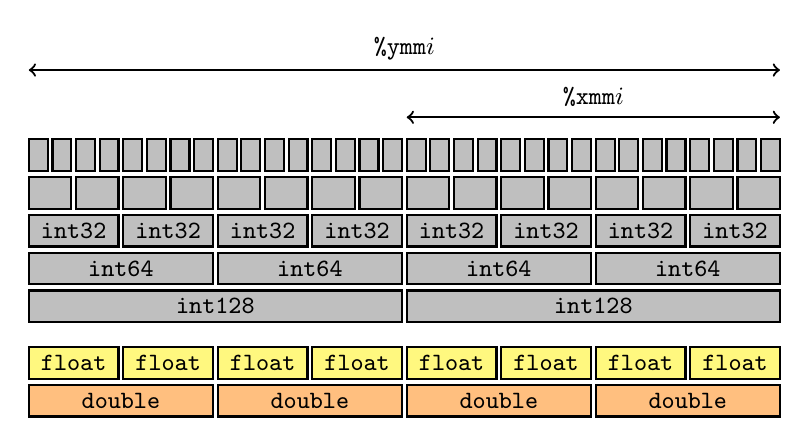
\begin{tikzpicture}[xscale=0.3, yscale=0.4, every node/.style={font=\small}]
  \foreach \i in {0, 8, 16, 24}
    \filldraw[thick, fill=orange, fill opacity=0.5] (\i, 0) rectangle +(7.8, 1);

  \foreach \i in {0, 4, ..., 31}
    \filldraw[thick, fill=yellow, fill opacity=0.5] (\i, 1.2) rectangle +(3.8, 1);

  \foreach \i in {0, 16}
    \filldraw[thick, fill=gray, fill opacity=0.5] (\i, 3) rectangle +(15.8, 1);

  \foreach \i in {0, 8, ..., 31}
    \filldraw[thick, fill=gray, fill opacity=0.5] (\i, 4.2) rectangle +(7.8, 1);

  \foreach \i in {0, 4, ..., 31}
    \filldraw[thick, fill=gray, fill opacity=0.5] (\i, 5.4) rectangle +(3.8, 1);

  \foreach \i in {0, 2, ...,  31}
    \filldraw[thick, fill=gray, fill opacity=0.5] (\i, 6.6) rectangle +(1.8, 1);

  \foreach \i in {0, 1, ...,  31}
    \filldraw[thick, fill=gray, fill opacity=0.5] (\i, 7.8) rectangle +(0.8, 1);

    \foreach \i in {0, 8, ..., 31}
    \path (\i, 0) rectangle node {\texttt{double}} +(7.8, 1);

    \foreach \i in {0, 4, ..., 31}
    \path (\i, 1.2) rectangle node {\texttt{float}} +(3.8, 1);

    \foreach \i in {0, 16}
    \path (\i, 3) rectangle node {\texttt{int128}} +(15.8, 1);

    \foreach \i in {0, 8, ..., 31}
    \path (\i, 4.2) rectangle node {\texttt{int64}} +(7.8, 1);

    \foreach \i in {0, 4, ..., 31}
    \path (\i, 5.4) rectangle node {\texttt{int32}} +(3.8, 1);

    \foreach \i in {0, 2, ..., 31}
    \path (\i, 6.6) rectangle  +(1.8, 1);

    \draw[thick,<->] (16, 9.5) -- node[above] {\texttt{\%xmm}$i$} +(15.8, 0);
    \draw[thick,<->] (0, 11) -- node[above] {\texttt{\%ymm}$i$} +(31.8, 0);
  \end{tikzpicture}

  \bigskip
  
\begin{tabular}{|c|c|c|}
  \hline
  Instructions & registers & size \\
  \hline\hline
  SSE$x$              & \texttt{\%xmm0}, \dots, \texttt{\%xmm15} & 128-bit \\
  \hline
  AVX + AVX2          & \texttt{\%ymm0}, \dots, \texttt{\%ymm15} & 256-bit \\
  \hline
  \multirow{2}{*}{AVX512} & \texttt{\%zmm0}, \dots, \texttt{\%zmm31} & 512-bit \\
               & \texttt{\%k0}, \dots, \texttt{\%k7}      & 64-bit \\
  \hline
  \end{tabular}
\end{center}
\end{frame}

%%%%%%%%%%%%%%%%%%%%%%%%%%%%%%%%%%%

\begin{frame}[fragile=singleslide]
  \frametitle{SIMD Instructions Nomenclature}
  
\red{Floating-point} SIMD instructions have compound names:
\begin{center}
  \verb|<prefix><op><simd or not><type>|
\end{center}
where
\begin{description}
\item[\texttt{<prefix>}:] empty (SSE), \texttt{v} (AVX, AVX2, AVX512)
\item[\texttt{<op>}] \texttt{add}, \texttt{sub}, \texttt{mul}, \texttt{div}, \texttt{fmadd}, \texttt{min}, \texttt{max}, \texttt{abs}, \texttt{floor}, \texttt{ceil}, \texttt{round}, \dots
\item[\texttt{<simd or not>}] \texttt{s} (\textit{scalar}), \texttt{p} (\textit{packed} --- i.e. vector).
\item[\texttt{<type>}] \texttt{s} (\textit{single}, \texttt{float}), \texttt{d} (\texttt{double})
\end{description}

\bigskip

E.g. \texttt{vmaxpd}, \texttt{vmulss}, etc.

\end{frame}

%%%%%%%%%%%%%%%%%%%%%%%%%%%%%%%%%%%%%%%%%%%%%%%%%%%%%%%%%%%%%%%%

\section{General Principles}

\begin{frame}
  \frametitle{Practical Vectorization}

  \begin{block}{General Principle}
    \begin{enumerate}
    \item Load data into vector registers
    \item Use vector instructions
    \item Write result back to memory
    \end{enumerate}
  \end{block}

  (minimizing these transfers is an important goal)
  
  \begin{alertblock}{Use cases}
    \begin{itemize}
    \item Happens \textbf{inside a \alert{single} thread}
      \begin{itemize}
      \item Parallelization = distribute over several cores
      \item Vectorization = use SIMD instructions inside \textbf{\red{ONE}} core
      \end{itemize}
    \item Only \textbf{small code chunks} can (usually) be vectorized
      \begin{itemize}
      \item Tight \textbf{loops} (limits of the instruction set) 
      \item [$\Rightarrow$] Target the \textbf{innermost} loops
      \end{itemize}
    \end{itemize}
  \end{alertblock}
\end{frame}  

%%%%%%%%%%%%%%%%%%%%%%%%%%%%%%%%%%%

\begin{frame}[fragile=singleslide]
  \frametitle{Obstacles}

  \begin{itemize}
  \item Data dependencies (dependent iterations)
     \begin{minted}{C}
     for (int i = 1; i < n; i++)
         a[i] += a[i-1];
\end{minted}
    \begin{itemize}
    \item No possible parallel processing 
      \item[$\hookrightarrow$] Must change the algorithm
    \end{itemize}

\medskip

\item Conditional instructions (\texttt{if})
     \begin{minted}{C}
     for (int i = 1; i < n; i++)
         if (a[i] != 0)
             a[i] = 1 / a[i];
\end{minted}
  \begin{itemize}
  \item Potentially manageable (overhead --- to avoid if possible)
  \end{itemize}

  \medskip

\item Complex memory access pattern and/or alignment problems 
  \begin{itemize}
  \item Loading \textbf{contiguous} array slices \red{only}
  \end{itemize}
  
  \medskip

\item Complex operations (sin, cos, log, exp, my\_function, ...)
\end{itemize}
\end{frame}  

%%%%%%%%%%%%%%%%%%%%%%%%%%%%%%%%%%%%%%%%%%%%%%

\begin{frame}[fragile=singleslide]
  \frametitle{Data Alignment}

  \begin{alertblock}{Rule of thumb}
    $xxx$-bytes vector must be located at an address multiple of $xxx$  
  \end{alertblock}

  \bigskip
  
  \begin{exampleblock}{Solutions}
    \begin{itemize}
    \item \mintinline{C}{double A[n] __attribute__ ((aligned(32)));}
      \begin{itemize}
      \item This is valid C code
      \end{itemize}
  \item \mintinline{C}{int posix_memalign(void **ptr, size_t align, size_t size);}
  \item \mintinline{C}{void *aligned_alloc(size_t alignment, size_t size);}
      \begin{itemize}
      \item Included in C11
      \end{itemize}
  \end{itemize}
\end{exampleblock}
\end{frame}

%%%%%%%%%%%%%%%%%%%%%%%%%%%%%%%%%%%%%%%%%%%%%%

\begin{frame}[fragile=singleslide]
  \frametitle{Complex memory access pattern}

\begin{alertblock}{Array of struct}
  \begin{minted}{C}
struct point {
      double x, y, z;
};

struct point *A;
  \end{minted}

\texttt{xyzxyzxyzxyzxyzxyz....}
\end{alertblock}

\begin{exampleblock}{Struct of Array}
  \begin{minted}{C}
struct points {
      double *x, *y, *z;
};
struct points A;          // facilitated batch processing
                          // arrays of uniform elements
  \end{minted}

  \texttt{xxxxxxxxxxxxxx....}\\
    \texttt{yyyyyyyyyyyyyy....}\\
    \texttt{zzzzzzzzzzzzzz....}\\
\end{exampleblock}

\end{frame}

%%%%%%%%%%%%%%%%%%%%%%%%%%%%%%%%%%%%%%%%%%%

\begin{frame}[fragile=singleslide]
  \frametitle{Vectorizing Simple Loops: \textit{strip-mining}}

  \begin{block}{Original code}
  \begin{minted}{C}
for (int i = 0; i < n; i++)
    u[i] = u[i] + alpha * v[i];
\end{minted}
\end{block}

\begin{exampleblock}{Transformed code}
\begin{minted}{C}
int m = n - (n % 4);
/* Processing in batches of 4 with SIMD instructions */
for (i = 0; i != m; i += 4) {
    u[i + 0] = u[i + 0] + alpha * v[i + 0];
    u[i + 1] = u[i + 1] + alpha * v[i + 1];
    u[i + 2] = u[i + 2] + alpha * v[i + 2];
    u[i + 3] = u[i + 3] + alpha * v[i + 3];
}
/* epilogue when n is not a multiple of 4 */
for (int i = m; i < n; i ++)
    u[i] = u[i] + alpha * v[i];
  \end{minted}
\end{exampleblock}
\begin{itemize}
\item Potentially: prologue to ensure alignment
\item The epilogue can be avoided with \textbf{padding}
\end{itemize}
\end{frame}

%%%%%%%%%%%%%%%%%%%%%%%%%%%%%%%%%%%%%%%%%%%%%%%%%%%%%%%%%%%%%

\begin{frame}
  \frametitle{\textit{strip-mining}?}

  \centering
  \includegraphics[width=10cm]{strip_mining.jpg}
\end{frame}

%%%%%%%%%%%%%%%%%%%%%%%%%%%%%%%%%%%%%%%%%%%%%%%%%%%%%%%%%%%%%%%

\begin{frame}[fragile=singleslide]
  \frametitle{Algorithmic Modifications }

  \begin{block}{Starting Point}

\begin{minted}{C}
double sum = 0;
for (int i = 0; i < n; i++)
    sum += a[i];               // data dependency (sum)
\end{minted}
  \end{block}

  \begin{exampleblock}{Transformed code}

\begin{minted}{C}
double __sum[4] = {0, 0, 0, 0};
for (int i = 0; i < n; i += 4) {      // assume that n is multiple of 4
    __sum[0] += a[i + 0];
    __sum[1] += a[i + 1];
    __sum[2] += a[i + 2];
    __sum[3] += a[i + 3];
}
// final reduction (non-vectorized)
double sum = __sum[0] + __sum[1] + __sum[2] + __sum[3];
\end{minted}

    \begin{itemize}
    \item Loop is now vectorizable
    \item Small overhead in epilogue
    \end{itemize}
  \end{exampleblock}
\end{frame}

%%%%%%%%%%%%%%%%%%%%%%%%%%%%%%%%%%%%%%%%%%%%%%%%%%%%%%%%%%%%%%%%

\begin{frame}[fragile]
  \frametitle{Apply a Full Sequential Algorithm on Vectors}

  \begin{columns}[T]
    \begin{column}{7cm}
  
      \begin{block}{Sequential Algorithm $\mathcal{A}$}
        \begin{itemize}
        \item Applies to an array $X$ 
        \item "\textit{data-oblivious}": sequence of instructions independent of the values
        \end{itemize}
      \end{block}

      \medskip

      \begin{exampleblock}<3->{Apply $k$ times the algorithm in parallel}
        \begin{itemize}
        \item scalars $\rightarrow$ vectors of size $k$
        \item scalar operations  $\rightarrow$ SIMD
        \end{itemize}
      \end{exampleblock}
    \end{column}

    \begin{column}{2.6cm}
  
      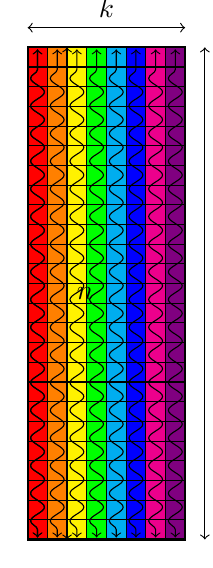
\begin{tikzpicture}[scale=0.25, line around/.style={decoration={pre length=#1,post length=#1}}]
        \path[use as bounding box] (0, 0) rectangle (8, 26);

        \fill<1-2>[fill=lightgray]  (0, 0) rectangle +(1, 25);
        \draw<1-2>[thick] (0, 0) rectangle (1, 25);
        
        \fill<3->[fill=red]     (0, 0) rectangle +(1, 25);
        \fill<3->[fill=orange]  (1, 0) rectangle +(1, 25);
        \fill<3->[fill=yellow]  (2, 0) rectangle +(1, 25);
        \fill<3->[fill=green]   (3, 0) rectangle +(1, 25);
        \fill<3->[fill=cyan]    (4, 0) rectangle +(1, 25);
        \fill<3->[fill=blue]    (5, 0) rectangle +(1, 25);
        \fill<3->[fill=magenta] (6, 0) rectangle +(1, 25);
        \fill<3->[fill=violet]  (7, 0) rectangle +(1, 25);
        \draw<3->[thick] (0, 0) rectangle (8, 25);
        \foreach \i in {1, 2, ..., 7}
        {
          \draw<3-> (\i, 0) -- +(0, 25);
        }

        \foreach \i in {1, 2, ..., 24}
        {
          \draw<1> (0, \i) -- +(1, 0);
          \draw<3>  (0, \i) -- +(8, 0);
        }

        
        \draw<1-2>[<->] (2, 0) -- node[right] {$n$} +(0, 25);

        \draw<3->[<->] (9, 0) -- node[right] {$n$} +(0, 25);
        \draw<3->[<->] (0, 26) -- node[above] {$k$} +(8, 0);
        
        \draw<2>[decorate, decoration=snake, line around=1mm, <->] (0.5, 0.1) -- +(0, 24.8);
        \foreach \i in {0, 1, 2, ..., 7}
        {
          \draw<4>[decorate, decoration=snake, line around=1mm, <->] (\i + 0.5 , 0.1) -- +(0, 24.8);
        }

      \end{tikzpicture}
    \end{column}
  \end{columns}
\end{frame}

%%%%%%%%%%%%%%%%%%%%%%%%%%%%%%%%%%%%%%%%%%%%%%%%%%%%%%%%%%%%%%%%

\section{Comment s'en servir ?}

\begin{frame}
  \frametitle{How to Use SIMD / Vector Instructions?}

  \begin{enumerate}
  \item \sout{Write assembler code directly}

    \medskip
    
  \item Use "\textit{instrinsics}" offered by compilers

\medskip
    
  \item Let the compiler do it (automatic vectorization)

\medskip
    
  \item Provide vectorization directives (OpenMP $\geq$ v4.0)

    \medskip
    
  \item Use \texttt{gcc}-specific vector extensions

  \end{enumerate}
\end{frame}


%%%%%%%%%%%%%%%%%%%%%%%%%%%%%%%%%%%%%%%% 
\subsection{intrinsics}

\begin{frame}[fragile=singleslide]
  \frametitle{Using the \emph{Intrinsics}}

  \begin{itemize}
  \item Introduced by Intel, later adopted by other compilers
  \item Pseudo-functions that emit \textbf{one} SIMD instruction
  \item Need to know the instruction set(s)
  \end{itemize}
  
  
\begin{block}{Headers}
  \begin{minted}{C}
#include <xmmintrin.h>         // SSE
#include <emmintrin.h>         // SSE2
#include <pmmintrin.h>         // SSE3
#include <tmmintrin.h>         // SSSE3
#include <smmintrin.h>         // SSE4.1
#include <nmmintrin.h>         // SSE4.2
#include <immintrin.h>         // AVX & AVX2 & AVX512
\end{minted}
\end{block}

\end{frame}

%%%%%%%%%%%%%%%%%%%%%%%%%%%%%%%%%%%%%%%%%%%%

\begin{frame}[fragile=singleslide]
  \frametitle{Data Types for the \emph{Intrinsics}}

\begin{block}{Match the hardware "vectors"}
  
  \begin{description}
  \item[\texttt{\_\_m512}] 512 bits (16 \texttt{float})
  \item[\texttt{\_\_m512d}] 512 bits (8 \texttt{double})
  \item[\texttt{\_\_m512i}] 512 bits (ints)
  \item + \texttt{\_\_mmask8}, \texttt{\_\_mmask16}, \texttt{\_\_mmask32}, \texttt{\_\_mmask64}
    
  \item[\texttt{\_\_m256}] 256 bits (8 \texttt{float})
  \item[\texttt{\_\_m256d}] 256 bits (4 \texttt{double})
  \item[\texttt{\_\_m256i}] 256 bits (ints)
    
  \item[\texttt{\_\_m128}] 128 bits (4 \texttt{float})
  \item[\texttt{\_\_m128d}] 128 bits (2 \texttt{double})
  \item[\texttt{\_\_m128i}] 128 bits (ints)
  \end{description}
\end{block}
\end{frame}

%%%%%%%%%%%%%%%%%%%%%%%%%%%%%%%%%%%%%%%%%%%% 

\begin{frame}[fragile=singleslide]
  \frametitle{Examples (AVX2)}

  \begin{itemize}
  \item \mintinline{C}{_mm256_set1_ps}
  \item \mintinline{C}{_mm256_load_pd}
  \item \mintinline{C}{_mm256_xor_si256}
  \item \mintinline{C}{_mm256_srli_epi32}
  \item \mintinline{C}{_mm256_i32gather_mask_pd}
  \item \mintinline{C}{_mm256_cmpeq_epi32}
  \item \mintinline{C}{_mm256_movemask_epi8}
  \item ...
  \end{itemize}
\end{frame}

%%%%%%%%%%%%%%%%%%%%%%%%%%%%%%%%%%%%%%%%%%%

\begin{frame}[fragile=singleslide]
  \frametitle{General Nomenclature}

  \begin{center}
    \verb|   _mm_<operation>_<suffix>(param1, param2)        |
    
    \verb|_mm256_<operation>_<suffix>(param1, param2, param3)|

    \verb|_mm512_<operation>_<suffix>(param1, param2, param3)|
  \end{center}

  \begin{block}{Two-part \texttt{<suffix>}}
    \begin{itemize}
    \item 1st part
      \begin{itemize}
      \item \texttt{p} (packed) and \texttt{ep} (extended packed): SIMD
      \item \texttt{s} (scalar): only 1st vector element is active 
      \end{itemize}

    
  \item 2nd part (type)
    \begin{itemize}
    \item{}  [\texttt{s}/\texttt{d}]: \textbf{s}ingle- or \textbf{d}ouble-precision float
    \item{} [\texttt{i}/\texttt{u}]\texttt{nnn}: s\textbf{i}gned or \textbf{u}nsigned \texttt{nnn}-bits integer \\ (\texttt{nnn} is 512, 256, 128, 64, 32, 16, or 8)
    \end{itemize}
  \end{itemize}
\end{block}
\end{frame}

%%%%%%%%%%%%%%%%%%%%%%%%%%%%%%%%%%%%%%%%%%%%%%

\begin{frame}[fragile=singleslide]
  \frametitle{Example}

  \begin{block}{Original Code}
\begin{minted}{C}
double alpha;
double u[], v[];
// ...
for (int i = 0; i < n; i++)
    u[i] = u[i] + alpha * v[i];
\end{minted}
\end{block}

\begin{exampleblock}{Vectorized code (AVX2)}
\begin{minted}{C}
__m256d valpha = _mm256_set1_pd(alpha);   // (alpha, alpha, alpha, alpha)
for (i = 0; i != m; i += 4) {
    /* processing by batches of 4 */
    __m256d vu = _mm256_load_pd(&u[i]);        // alignment required
    __m256d vv = _mm256_load_pd(&v[i]);        // alignment required
    __m256d vres = _mm256_fmadd_pd(valpha, vv, vu);
    _mm256_store_pd(&u[i], vres);              // alignment required
}
  \end{minted}
\end{exampleblock}
\end{frame}

%%%%%%%%%%%%%%%%%%%%%%%%%%%%%%%%%%%%%%%%%%%%%%%% 

\begin{frame}[fragile=singleslide]
  \frametitle{Non-Trivial Example: Colorimetric Conversions}

  \centering
  \includegraphics[width=10cm]{rgb_cmyk.png}
\end{frame}

%%%%%%%%%%%%%%%%%%%%%%%%%%%%%%%%%%%%%%%%%%%%%%%

\begin{frame}[fragile=singleslide]
  \frametitle{Non-Trivial Example: Colorimetric Conversions}

  R, G, B, C, M, Y, K = floats in $[0; 1]$

  \begin{exampleblock}{Easy Direction}
  \[
  \left\{
    \begin{array}{rl}
      R &= (1-C) \times (1 - K) \\
      G &= (1-M) \times (1 - K) \\
      B &= (1-Y) \times (1 - K)
    \end{array}
    \right.
\]
\end{exampleblock}

\begin{alertblock}{Problematic direction}
  \begin{itemize}
  \item If $(R, G, B) = (0, 0, 0)$ then $(C,M,Y,K) = (0, 0, 0, 1)$
    
  \item Otherwise
    \[  \left\{\begin{array}{rl}
      K &= 1 - \max(R, G, B) \\
      C &= 1 - R  / (1 - K) \\
      M &= 1 - G  / (1 - K) \\
      Y &= 1 - B  / (1 - K) 
    \end{array}
    \right.
\]
\end{itemize}


\end{alertblock}
\end{frame}

%%%%%%%%%%%%%%%%%%%%%%%%%%%%%%%%%%%%%%%%%%%%%%%%%%%%%%%%%%%%%%%%%%%%%%%%%%%%%

\begin{frame}[fragile=singleslide]
  \frametitle{Problems with Conditional Instructions}
  \framesubtitle{Example: RGB $\rightarrow$ CMYK}

  \begin{block}{$K = 1 - \max(R, G, B)$}
\begin{minted}{C}
__m256 vone = _mm256_set1_ps(1.0);            // (1, 1, 1, 1, 1, 1, 1, 1)
// ...
/* process a chunk of 8 colors */
__m256 vR = _mm256_load_ps(&R[i]);               // alignment required
__m256 vG = _mm256_load_ps(&G[i]);               // alignment required
__m256 vB = _mm256_load_ps(&B[i]);               // alignment required
__m256 vmax = _mm256_max_ps(_mm256_max_ps(vR, vG), vB);
__m256 vK = _mm256_sub_ps(vone, vmax);
_mm256_store_ps(&K[i], vk);                      // alignment required
\end{minted}
\end{block}

  \begin{alertblock}{If $K < 1$}
\begin{minted}{C}
__m256 vC = _mm256_sub_ps(vone, _mm256_div_ps(vR, vmax));
__m256 vM = _mm256_sub_ps(vone, _mm256_div_ps(vG, vmax));
__m256 vY = _mm256_sub_ps(vone, _mm256_div_ps(vB, vmax));
\end{minted}
  \end{alertblock}  
\end{frame}

%%%%%%%%%%%%%%%%%%%%%%%%%%%%%%%%%%%%%%%%%%%%%%%%%%%%%%%%%%%%%%%%%%%%%%%%%%%

\begin{frame}[fragile=singleslide]
  \frametitle{Problems with Conditional Instructions}
  \framesubtitle{Example: RGB $\rightarrow$ CMYK}

  \begin{exampleblock}{If $K = 1$}
\begin{minted}{C}
    __m256 vzero = __m256 _mm256_setzero_ps();
    __m256 vmask = _mm256_cmp_ps(vK, vone, _CMP_EQ_OQ);
    // vmask[i] == (vK[i] == 1.0) ? 0xffffffff : 0x00000000 
    vC = _mm256_blendv_ps(vzero, vC, vmask);
    vM = _mm256_blendv_ps(vzero, vM, vmask);
    vY = _mm256_blendv_ps(vzero, vY, vmask);
    // blendv : vX[i] =     vmask[i]   ? vzero[i] : vX[i]
    //                  (vK[i] == 1.0) ? vzero[i] : vX[i]   
\end{minted}
  \end{exampleblock}

  \begin{block}{Intructions for shuffling data inside registers:}
  \begin{itemize}
  \item \texttt{blend}, \texttt{blendv}, \texttt{broadcast}, \texttt{extract}, \texttt{insert}, \texttt{permute},  \texttt{permutevar}, \texttt{shuffle}, \texttt{unpackhi}, \texttt{unpacklo}, ...
  \end{itemize}
\end{block}
\end{frame}

%%%%%%%%%%%%%%%%%%%%%%%%%%%%%%%%%%%%%%%%%%%%%%%%%%%%%%%%%%%%%%%%%%%%%%

\begin{frame}[fragile=singleslide]
  \frametitle{Problems with Conditional Instructions}
  \framesubtitle{Example: RGB $\rightarrow$ CMYK}

\begin{minted}{C}
// R, G, B, C, M, Y, K must be aligned
__m256 vone, vzero, vmask, vR, vG, vB, vC, vM, vY, vK;
vone = _mm256_set1_ps(1.0);            // (1, 1, 1, 1, 1, 1, 1, 1)
vzero = _mm256_setzero_ps();           // (0, 0, 0, 0, 0, 0, 0, 0)
for (int i = 0; i < n; i += 8) {
    vR = _mm256_load_ps(&R[i]);
    vG = _mm256_load_ps(&G[i]);
    vB = _mm256_load_ps(&B[i]);
    vmax = _mm256_max_ps(_mm256_max_ps(vR, vG), vB);
    vK = _mm256_sub_ps(vone, vmax);
    vC = _mm256_sub_ps(vone, _mm256_div_ps(vR, vmax));
    vM = _mm256_sub_ps(vone, _mm256_div_ps(vG, vmax));
    vY = _mm256_sub_ps(vone, _mm256_div_ps(vB, vmax));
    vmask = _mm256_cmp_ps(vK, vone, _CMP_EQ_OQ);
    vC = _mm256_blendv_ps(vzero, vC, vmask);
    vM = _mm256_blendv_ps(vzero, vM, vmask);
    vY = _mm256_blendv_ps(vzero, vY, vmask);
    _mm256_store_ps(&C[i], vC);
    _mm256_store_ps(&M[i], vM);
    _mm256_store_ps(&Y[i], vY);
    _mm256_store_ps(&K[i], vK);
}
\end{minted}
\end{frame}

\subsection{OpenMP}

%%%%%%%%%%%%%%%%%%%%%%%%%%%%%%%%%%%%%%%%%%%

\begin{frame}[fragile=singleslide]
  \frametitle{OpenMP \texttt{simd} Directive}

  \begin{alertblock}{OpenMP reminder}
    \begin{itemize}
    \item requires compiling with \texttt{-fopenmp}
    \item \texttt{-fopenmp-simd} enables SIMD but not threads
    \end{itemize}
  \end{alertblock}
  
  \bigskip
  
  \begin{minted}{C}
    #pragma omp simd
    for (int i = 0; i < n; i++)
       ...
  \end{minted}

  \begin{itemize}
  \item Groupe iterations in \textit{chunks} of size $N$
    \begin{itemize}
    \item Do the computation using $N$-wide SIMD instructions
    \end{itemize}
    
  \item We ``promise'' the compiler that the loop is vectorizable
  \item No multi-thread parallelization there
  \end{itemize}
\end{frame}

%%%%%%%%%%%%%%%%%%%%%%%%%%%%%%%%%%%%%%%% 

\begin{frame}[fragile=singleslide]
  \frametitle{OpenMP \texttt{simd} Directive}
  
  \begin{minted}{C}
    #pragma omp simd [clause[[,] clause],...]
    for (int i = 0; i < n; i++)
        ...
   \end{minted}

   \begin{block}{Possible clauses (non-exhaustive list)}
     \begin{itemize}
     \item \texttt{reduction(+:v}): already known 
       \begin{itemize}
       \item Breaks data dependency on accumulator variable
       \end{itemize}
       \smallskip
       
     \item \texttt{simdlen(length)}: desired \textit{chunk} size
\smallskip
       
     \item \texttt{safelen(length)}: maximum allowed \textit{chunk} size
       \begin{itemize}
       \item E.g., beyond this a dependency problem could occur
       \end{itemize}
\smallskip
       
     \item \texttt{aligned(v[:k])}: promise that $v$ is aligned on \texttt{k} bytes
\smallskip


     \item \texttt{linear(x[:step])}: $x$ is an affine function of $i$ (\mintinline{C}{x_i = x_init + i * step;})
     \end{itemize}
   \end{block}
 \end{frame}


\subsection{Vectorisation auto}

%%%%%%%%%%%%%%%%%%%%%%%%%%%%%%%%%%%%%%%%%%%%%%%%%%%%%%%%%%%%%%%%%%%%%%%

\begin{frame}[fragile=singleslide]
  \frametitle{Automatic Vectorization }

  \begin{itemize}
  \item Fortran a has explicit vectors
    \begin{itemize}
    \item Easy to vectorize
    \end{itemize}
    \item In C, compiler detects \textbf{vectorizable loops}

  \end{itemize}

\begin{exampleblock}{C Code}
\begin{minted}{C}
for (int i = 0; i < n; i++)
        C[i] = lambda * A[i] + mu * B[i];
\end{minted}
\end{exampleblock}

\begin{alertblock}{Assembler code produced by \texttt{gcc}}

\begin{minted}{gas}
.loop:
        vmulpd  (%rsi,%rax), %ymm3, %ymm0    
        vmulpd  (%rcx,%rax), %ymm2, %ymm1
        vaddpd  %ymm1, %ymm0, %ymm0
        vmovapd %ymm0, (%rdx,%rax)
        addq    $32, %rax
        cmpq    %rcx, %rax
        jne     .loop
\end{minted}
\end{alertblock}%$
\end{frame}


%%%%%%%%%%%%%%%%%%%%%%%%%%%%%%%%%%%%%%%%%%%%%%%%%%%%%%%%%%%%%%%%%

\begin{frame}[fragile=singleslide]
  \frametitle{SIMD Instructions in \texttt{gcc}}

    \begin{itemize}
    \item \textbf{automatic vectorization} is \alert{disabled} by default 
      \begin{itemize}
      \item Without explicit options, ``optimization level'' = 0
      \item automatic vectorization (and OpenMP) disabled
      \end{itemize}

      \medskip
      
    \item Enable with option \verb|-ftree-vectorize|
      \begin{itemize}
      \item \verb|-O3| activates this feature
      \end{itemize}
    \item We're doing HPC: always compile with \verb|-O2| or \verb|-O3|
  \begin{minted}{shell}
~$ gcc -O1 -ftree-vectorize vectorisation_auto.c
~$ gcc -O1 -fopenmp vectorisation_omp.c
\end{minted}

\medskip
  
  \item \texttt{gcc} does \textbf{not} emit AVX2 (resp. FMA) instructions by default
    \begin{itemize}
    \item Add \verb|-mavx2| (resp. \verb|-mfma|) to the command-line
    \end{itemize}

\medskip

\item Verbosity and diagnostics:
  \begin{itemize}
  \item \scriptsize \verb|-fopt-info-vec|, \verb|-fopt-info-vec-missed| and \verb|-fopt-info-vec-all|
  \end{itemize}
  \end{itemize}

  
    % Il n'est très simple de vérifier si les bonnes instructions vectorielles sont utilisées, mais on peut tenter de désassembler le binaire produit à leur recherche. Par exemple, pour vérifier l'utilisation de l'instruction mulps :

    % 		objdump -d ./executable | grep mulps
\end{frame}

%%%%%%%%%%%%%%%%%%%%%%%%%%%%%

\section{FFT}

\begin{frame}
  \frametitle{Case Study}

  \begin{block}{\textbf{Discrete Fourier Transform} (DFT)}
  \begin{itemize}
  \item The DFT of an array $X$ of $n$ (complexes) numbers is
\[
  Y[k] = \sum_{j=0}^{n-1} X[j] \omega_n^{jk}, \qquad \text{with} \qquad \omega_n = e^{-\frac{2i\pi}{n}} \qquad (0 \leq k < n)
\]
\item Optimized libraries (e.g. FFTW)
\end{itemize}
\end{block}

\medskip

\begin{alertblock}{Rewriting the definition}
When $n = n_1 \times n_2$, we set
$j = j_1 n_2 + j_2$ and $k = k_1 + k_2 n_1$ 
\[
Y[k_1 + k_2 n_1] = \sum_{j_2 = 0}^{n_2 - 1} \left[ \left( \sum_{j_1 = 0}^{n_1 - 1} X[j_1n_2 + j_2] {\omega_{n_1}}^{j_1 k_1} \right) {\omega_n}^{j_2 k_1} \right] {\omega_{n_2}}^{j_2 k_2}
\]
\end{alertblock}

\end{frame}

%%%%%%%%%%%%%%%%%%%%%%%%%%%%%%%%%%%%%%%%%%%%%%%%%%%%%%%

\begin{frame}
  \frametitle{FFT: Recursive Algorithm}

$n = n_1 \times n_2$, we set $j = j_1 n_2 + j_2$ et $k = k_1 + k_2 n_1$ 

\[
Y[k_1 + k_2 n_1] = \sum_{j_2 = 0}^{n_2 - 1} \left[ \left( \sum_{j_1 = 0}^{n_1 - 1} X[j_1n_2 + j_2] {\omega_{n_1}}^{j_1 k_1} \right) {\omega_n}^{j_2 k_1} \right] {\omega_{n_2}}^{j_2 k_2}
\]
  
\begin{block}{Algorithm to compute the DFT of size $n_1 \times n_2$}
  \begin{enumerate}
  \item Do $n_2$ DFTs of size $n_1$ (internal sum)
  \item Multiply by the \emph{twiddle factors} ${\omega_n}^{j_2 k_1}$
  \item Do $n_1$ DFTs of size $n_2$ (external sum)
  \end{enumerate}
\end{block}

\end{frame}

%%%%%%%%%%%%%%%%%%%%%%%%%%%%%%%%%%%%%%%%%%%%%%%%%%%%%%%%%%%

\begin{frame}[fragile]
  \frametitle{FFT: Recursive Algorithm}
  \framesubtitle{Classical Presentation}

    \begin{columns}[T]
    \begin{column}{8cm}

      \begin{itemize}
      \item Common choice : $n_2 = 2$
        \begin{itemize}
        \item ``\textit{Radix-2 Decimation in Time}''
        \end{itemize}
        
      \item FFT of size 2 : $(x, y) \rightarrow (x + y, x - y)$
      \end{itemize}
      
      
\begin{minted}{C}
void FFT(const double * X, double *Y, int n, int s)
{
    if (n == 1) {
       Y[0] = X[0];
       return;
    }
    double omega_n = exp(-2*I*pi / n);
    double omega = 1;   // twiddle factor
    FFT(&X[0], &Y[0]  , n/2, 2*s);
    FFT(&X[s], &Y[n/2], n/2, 2*s);
    for (int i = 0; i < n/2; i++) {
        double p = Y[i];
        double q = Y[i + n/2] * omega;
        Y[i] = p + q;
        Y[i + n/2] = p - q;
        omega *= omega_n;    
    }
}
\end{minted}

    \end{column}
    \begin{column}{1.6cm}
    
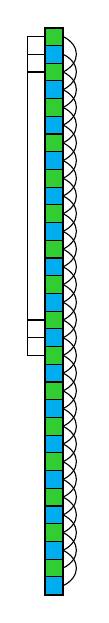
\begin{tikzpicture}[scale=0.225,line around/.style={decoration={pre length=#1,post length=#1}}]
  \path[use as bounding box] (-1, 0) rectangle (2, 32);
  \foreach \i in {0, 2, ..., 30}
  {
    \fill[fill=cyan] (0, \i) rectangle +(1, 1);
    \fill[fill=LimeGreen] (0, \i + 1) rectangle +(1, 1);
  }
  \draw[thick] (0, 0) rectangle (1, 32);
  \foreach \i in {0, 1, ..., 31}
  {
    \draw (0, \i) -- +(1, 0);
  }

  \foreach \j in {1, 3, ..., 29}
  {
    \draw<2> (1, \j + 0.5) .. controls (2, \j + 1) and (2, \j + 2) .. (1, \j + 2.5);
  }
  \foreach \j in {0, 2, ..., 28}
  {
    \draw<3> (1, \j + 0.5) .. controls (2, \j + 1) and (2, \j + 2) .. (1, \j + 2.5);
  }

  \draw<4> (0, 31.5) -- (-1, 31.5) -- (-1, 15.5) -- (0, 15.5);
  \draw<5> (0, 30.5) -- (-1, 30.5) -- (-1, 14.5) -- (0, 14.5);
  \draw<6> (0, 29.5) -- (-1, 29.5) -- (-1, 13.5) -- (0, 13.5);

\end{tikzpicture}
\end{column}
\end{columns}
\end{frame}

%%%%%%%%%%%%%%%%%%%%%%%%%%%%%%%%%%%%%%%%%%%%%%%%%%%%%%%%%%% 

\begin{frame}[fragile]
  \begin{overlayarea}{\textwidth}{2cm}
      
  \only<1-3>{
    \[
      Y[k_1 + k_2 n_1] = \sum_{j_2 = 0}^{n_2 - 1} \left[ \left( \sum_{j_1 = 0}^{n_1 - 1} X[j_1n_2 + j_2] {\omega_{n_1}}^{j_1 k_1} \right) {\omega_n}^{j_2 k_1} \right] {\omega_{n_2}}^{j_2 k_2}
    \]
  }
  \only<4>{
    \[
      Y[k_1 + k_2 n_1] = \sum_{j_2 = 0}^{n_2 - 1} \left( U[k_1 n_2 + j_2] {\omega_n}^{j_2 k_1} \right) {\omega_{n_2}}^{j_2 k_2}
    \]
  }
  \only<5->{
    \[
      Y[k_1 + k_2 n_1] = \sum_{j_2 = 0}^{n_2 - 1} V[k_1 n_2 + j_2] {\omega_{n_2}}^{j_2 k_2}
    \]
  }
\end{overlayarea}

\begin{overlayarea}{\textwidth}{8cm}
  \begin{columns}[T]
    \begin{column}{6cm}
      \small 
      \begin{itemize}
      \item<2-> $U[\star, j_2] \gets FFT(X[\star, j_2])$
        \begin{itemize}
        \item $0 \leq j_2 < n_2$
        \end{itemize}

      \item<4-> $V[k_1, j_2] \gets U[k_1, j_2] \cdot {\omega_n}^{j_2 k_1}$
        \begin{itemize}
        \item $0 \leq j_2 < n_2$
        \item $0 \leq k_1 < n_1$ 
        \end{itemize}

      \item<7-> Transpose $V$
        \begin{itemize}
        \item \red{overhead} from vectorization
        \end{itemize}
        
      \item<only@5-6> $Y[k_1, \star] \gets FFT(V[k_1, \star])$
        \begin{itemize}
        \item $0 \leq k_1 < n_1$
        \end{itemize}

      \item<8-> $Y[\star, k_1] \gets FFT(V[\star, k_1])$
        \begin{itemize}
        \item $0 \leq k_1 < n_1$
        \end{itemize}

      \item<10-> Retranspose $Y$
        \begin{itemize}
        \item \red{overhead} from vectorization
        \end{itemize}
        
      \end{itemize}
    \end{column}

    \begin{column}{5.8cm}
      \begin{tikzpicture}[scale=0.25,line around/.style={decoration={pre length=#1,post length=#1}}]
        \path[use as bounding box] (0, 0) rectangle (20, 22);

        \draw<1-6,10>[<->] (9, 0) -- node[right] {$n_1$} +(0, 20);
        \draw<1-6,10>[<->] (0, 21) -- node[above] {$n_2$} +(8, 0);
        \fill<1>[fill=lightgray] (0, 0) rectangle (8, 20);
        \fill<2-6>[fill=red]      (0, 0) rectangle +(1, 20);
        \fill<2-6>[fill=orange]   (1, 0) rectangle +(1, 20);
        \fill<2-6>[fill=yellow]   (2, 0) rectangle +(1, 20);
        \fill<2-6>[fill=green]    (3, 0) rectangle +(1, 20);
        \fill<2-6>[fill=cyan]     (4, 0) rectangle +(1, 20);
        \fill<2-6>[fill=blue]     (5, 0) rectangle +(1, 20);
        \fill<2-6>[fill=magenta]  (6, 0) rectangle +(1, 20);
        \fill<2-6>[fill=violet]   (7, 0) rectangle +(1, 20);
        \draw<1-6,10>[thick] (0, 0) rectangle (8, 20);
        \foreach \i in {1, 2, ..., 7}
        {
          \draw<1,2,3,4> (\i, 0) -- +(0, 20);
        }
        \foreach \j in {1, 2, ..., 19}
        {
          \draw<1,2,4,5,6> (0, \j) -- +(8, 0);
        }

        % transposée
        \draw<7-9>[<->] (21, 0) -- node[right] {$n_2$} +(0, 8);
        \draw<7-9>[<->] (0, 9) -- node[above] {$n_1$} +(20, 0);
        \fill<7-8>[fill=red]      (0, 7) rectangle +(20, 1);
        \fill<7-8>[fill=orange]   (0, 6) rectangle +(20, 1);
        \fill<7-8>[fill=yellow]   (0, 5) rectangle +(20, 1);
        \fill<7-8>[fill=green]    (0, 4) rectangle +(20, 1);
        \fill<7-8>[fill=cyan]     (0, 3) rectangle +(20, 1);
        \fill<7-8>[fill=blue]     (0, 2) rectangle +(20, 1);
        \fill<7-8>[fill=magenta]  (0, 1) rectangle +(20, 1);
        \fill<7-8>[fill=violet]   (0, 0) rectangle +(20, 1);
        \draw<7-9>[thick] (0, 0) rectangle (20, 8);
        \foreach \i in {1, 2, ..., 7}
        {
          \draw<7> (0, \i) -- +(20, 0);
        }
        \foreach \j in {1, 2, ..., 19}
        {
          \draw<7,8> (\j, 0) -- +(0, 8);
        }

        
        % 1ère passe FFT
        \foreach \i in {0, 1, 2, ..., 7} {
          \draw<3>[decorate,decoration=snake, line around=1mm,<->] (\i + 0.5, 0.1) -- +(0, 19.8);
        }
               
        % twiddle
        \foreach \i in {0.5, 1.5, ..., 7.5} {
          \foreach \j in {0.5, 1.5, ..., 19.5} {
            \draw<4>[black,variable=\t,smooth,domain=0:19.5,samples=20] (\i, \j) plot ({\i + 0.0225 * \t *sin(\t r)}, {\j + 0.0225 * \t * cos(\t r)});
          }
        }

        % 2ème passe FFT (avortée)
        \foreach \i in {0, 1, 2, ..., 19} {
          \draw<5,6>[decorate,decoration=snake, line around=1mm,<->] (0.1, \i + 0.5) -- +(7.8, 0);
        }
        \draw<6>[line width=2mm, black] (-1, -1) -- (9, 21); 
        \draw<6>[line width=2mm, black] (-1, 21) -- (9, -1); 

        % 2ème passe FFT (réussie)
        \foreach \i in {0, 1, 2, ..., 19} {
          \draw<8>[decorate,decoration=snake, line around=1mm,<->] (\i + 0.5, 0.1) -- +(0, 7.8);
        }

        % à transposer
        \node<9> at (10, 4) {\includegraphics[height=2cm]{Triste.png}};
        \node<10> at (4, 10) {\includegraphics[width=2cm]{Content.png}};

      \end{tikzpicture}
    \end{column}
  \end{columns}
\end{overlayarea}
\end{frame}

%%%%%%%%%%%%%%%%%%%%%%%%%%%%%%%%%%%%%%%

\begin{frame}
  \frametitle{Addendum: Vectorized Transposition}

    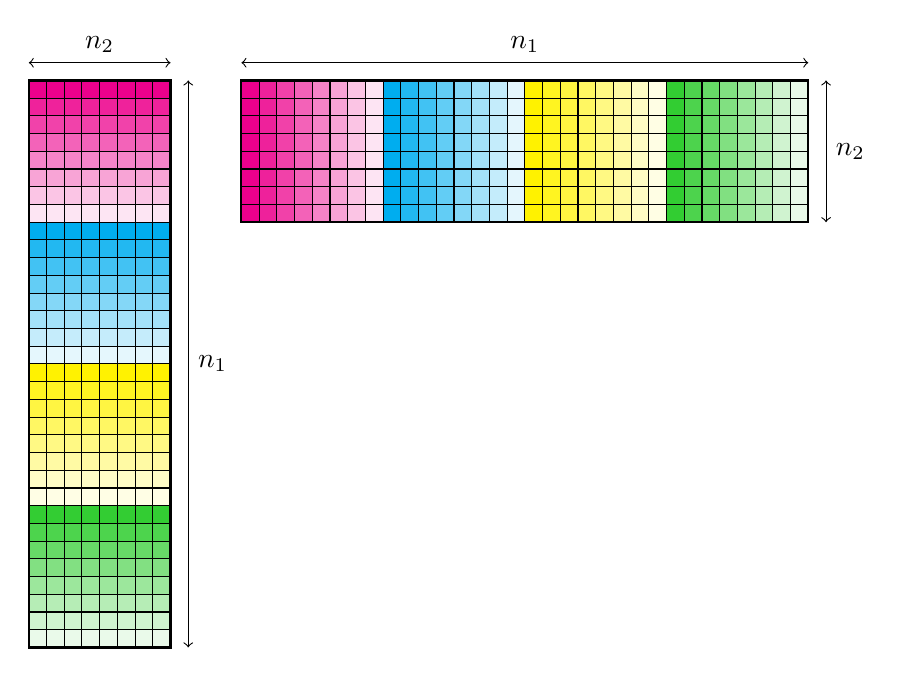
\begin{tikzpicture}[scale=0.225]
%        \path[use as bounding box] (0, 0) rectangle (20, 22);

        \draw[<->] (9, 0) -- node[right] {$n_1$} +(0, 32);
        \draw[<->] (0, 33) -- node[above] {$n_2$} +(8, 0);

        \foreach \i in {0, ..., 7}
        {
          \fill[fill=LimeGreen, fill opacity=0.1 + \i*0.128] (0, \i)      rectangle +(8, 1);
          \fill[fill=yellow,    fill opacity=0.1 + \i*0.128] (0, \i + 8)  rectangle +(8, 1);
          \fill[fill=cyan,      fill opacity=0.1 + \i*0.128] (0, \i + 16) rectangle +(8, 1);
          \fill[fill=magenta,   fill opacity=0.1 + \i*0.128] (0, \i + 24) rectangle +(8, 1);
        }
        \foreach \i in {1, ..., 7}
        {
          \draw (\i, 0) -- +(0, 32);
        }
        \foreach \j in {1, 2, ..., 31}
        {
          \draw (0, \j) -- +(8, 0);
        }
        \draw[thick] (0, 0) rectangle (8, 32);

        
        \begin{scope}[xshift=12cm, yshift=24cm]
        % transposée
        \draw[<->] (33, 0) -- node[right] {$n_2$} +(0, 8);
        \draw[<->] (0, 9) -- node[above] {$n_1$} +(32, 0);

        \foreach \i in {0, ..., 7}
        {
          \fill[fill=magenta,   fill opacity=1 - \i*0.128] (\i     , 0) rectangle +(1, 8);
          \fill[fill=cyan,      fill opacity=1 - \i*0.128] (\i +  8, 0) rectangle +(1, 8);
          \fill[fill=yellow,    fill opacity=1 - \i*0.128] (\i + 16, 0) rectangle +(1, 8);
          \fill[fill=LimeGreen, fill opacity=1 - \i*0.128] (\i + 24, 0) rectangle +(1, 8);
        }
        \foreach \i in {1, ..., 7}
        {
          \draw (0, \i) -- +(32, 0);
        }
        \foreach \j in {1, 2, ..., 31}
        {
          \draw (\j, 0) -- +(0, 8);
        }
        \draw[thick] (0, 0) rectangle (32, 8);
      \end{scope}  
    \end{tikzpicture}

    \begin{textblock}{8}(5.5, 9)
      \begin{block}{``Fun'' exercise}
        Write code that transpose 
        \begin{itemize}
        \item A $4 \times 4$ matrix of \texttt{double}
        \item A $8 \times 8$ matrix of \texttt{float}
        \item Using \emph{intrinsics}
        \end{itemize}
      \end{block}
    \end{textblock}
    
\end{frame}

\end{document}


%%% Local Variables:
%%% TeX-command-extra-options: "-shell-escape"
%%% TeX-engine: xetex
%%% ispell-local-dictionary: "english"
%%% eval: (flyspell-mode 1)
%%% eval: (reftex-mode 1)
%%% End:
